\appendix

%%%%%%%%%%%%%%%%%%%%%%%%%%%%%%%%%%%%%%%%%%%%%%%%
% Apendice A
%%%%%%%%%%%%%%%%%%%%%%%%%%%%%%%%%%%%%%%%%%%%%%%%
\chapter{Edad escolar en diferentes Sistemas Educativos}\label{anexo:edad-educacion}

Incluso en la Unión Europea, los Sistemas Educativos difieren en la edad de escolarización de los estudiantes. Por ello, se ha confeccionado una tabla que intenta resumir la edad estándar en la que un niño está escolarizado durante las distintas etapas educativas\footnote{Se hablará de las etapas en las que el Sistema Educativo referido está bajo la responsabilidad del Ministerio de Educación (o equivalente) del propio país. Esto no excluye a la educación en centros privados.}. La información que se muestra a continuación está basado en \cite{cursos-educacion-europa} y \cite{guide-education-us}.

Se tomarán como referencia los nombres de las etapas del Sistema Educativo Español (Educación Infantil, Primaria, Secundaria y Bachillerato) para mostrar los años que pasan los estudiantes. Con respecto a la selección de países para realizar la comparación, se escogen los más representativos en los que se han realizado los estudios sobre el aprendizaje de la programación y donde más extendido están las plataformas que se mencionan en el presente documento. 


\begin{table}[!ht]
	\begin{centering}
		\begin{tabular}{c|c|c|c|c}
\emph{País} & Infantil & Primaria & Secundaria & Bachillerato\\
\hline
\emph{España} & 0-6 & 6-12 & 12-16 & 16-18\\
\emph{Estados Unidos} & 3-6 & 6-10 & 10-14 & 14-18\\
\emph{Reino Unido} & 2-5 & 5-11 & 11-16 & 16-18\\
\emph{Alemania} & 0-6 & 6-10 & 10-16 & 16-19\\
\emph{Francia} & 2-6 & 6-11 & 11-16 & 16-18\\
\emph{Bélgica} & 0-2.5/3 & 2.5/3-6 & 6-12 & 12-18\\
\emph{Irlanda} & 4-6 & 6-12 & 12-15 & 15-19\\
\end{tabular}
	\caption{Comparativa de edades de escolarización en diferentes Sistemas Educativos con respecto a las etapas del Sistema Educativo Español.}
		\label{tab:comparativa-tecnicas}
	\end{centering}
\end{table}

En el caso del Sistema Educativo Americano, existen muchas vías en la formación de un niño, como bien detalla A. Corsi-Bunker en \cite{guide-education-us}. Dependiendo de si se escoge una vía privada o dependiendo del estado, los años pueden variar. Aún así, en la figura \ref{tab:comparativa-tecnicas} se muestra el modelo estándar (sistema K-12).\footnote{Para más información sobre el Sistema Educativo Americano recomiendo que se acuda directamente a la fuente: U.S. Department of Education, National Center for Education Statistics (\url{http://nces.ed.gov})}.

\begin{figure}[!ht]
	\begin{centering}
		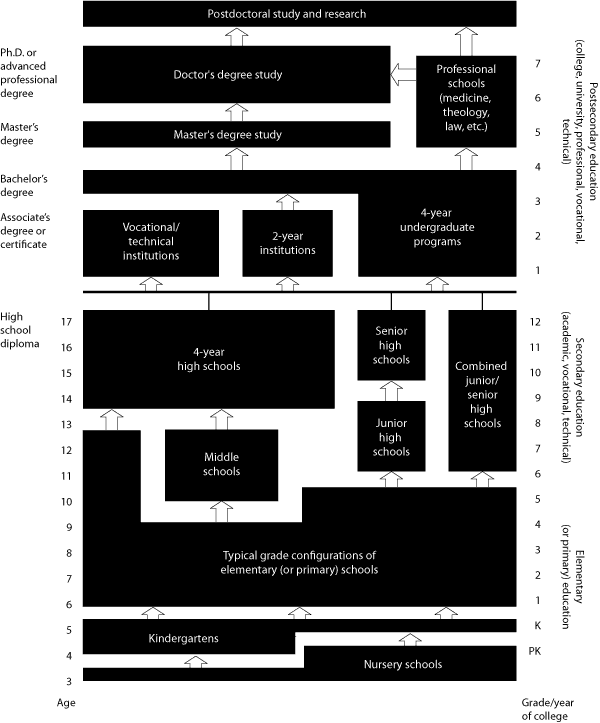
\includegraphics[width=0.75\textwidth]{images/education-usa.png}
			\caption{Tabla que muestra los típicos patrones de progresión en el Sistema Educativo Americano. Fuente: U.S. Department of Education, National Center for Education Statistics, Annual Reports Program. Obtenido de \url{http://nces.ed.gov/programs/digest/d11/figures/fig_01.asp}}
				\label{fig:education-usa}
	\end{centering}
\end{figure}





%%%%%%%%%%%%%%%%%%%%%%%%%%%%%%%%%%%%%%%%%%%%%%%%
% Apendice B
%%%%%%%%%%%%%%%%%%%%%%%%%%%%%%%%%%%%%%%%%%%%%%%%
\chapter{Lenguaje Logo}
\label{anexo:logo-lenguaje}

A continuación se realizará una revisión de las principales características del lenguaje Logo para tener una visión general de su funcionamiento y sintaxis. Este análisis se basa en el trabajo de \cite[p.274-305]{feurzeig1969programming}. Si el lector quiere ampliar información sobre el lenguaje Logo, puede consultar \cite{friendly2014advanced} o \cite{logo-resources}.


\section*{\emph{words}, \emph{sentences}, operaciones y comandos}

Hay dos tipos de datos principales: \emph{words} y \emph{sentences}. \emph{words} está formado por 0 o más caracteres, sin espacios. Algunos ejemplos son: "SUN", "CAT", "5",  "97&!", "" (cadena vacía). El tipo de datos \emph{sentences} se forma por un conjunto de \emph{words} separado por espacios, como por ejemplo "HELLO WORLD" o "3 + 2 = 5". Un numero es una \emph{word} pero conpuesto únicamente por dígitos.

En el lenguaje Logo existen operadores para tratar con los tipos \emph{words} y \emph{sentences}. También se pueden encontrar una serie de operaciones predefinidas en el lenguaje que ofrecen funcionalidad extra, como controlar la entrada/salida de un programa, saber la fecha o manejo de \emph{words} y \emph{sentences}. En la tabla \ref{tab:logo-operaciones} vemos un resumen de las operaciones elementales del lenguaje Logo, el número de argumentos que requiere y un ejemplo de entrada con su salida correspondiente.


\begin{table}[!ht]
	\begin{centering}
		\begin{tabular}{c|c|c|c}
\emph{Operador} & N. argumentos & Entrada & Salida\\
\hline
\texttt{FIRST}	& 1 & "CAT" & "C"\\
- & - & "CAT AND DOG" & "CAT"\\
\texttt{LAST} & 1 & "CAT" & "T"\\
- & - & "CAT AND DOG" & "DOG"\\
\texttt{BUTFIRST} &1& "CAT" & "AT"\\
- & - & "CAT AND DOG" & "AND DOG"\\
\texttt{BUTLAST} & 1 & "CAT" & "CA"\\
- & - & "CAT AND DOG" & "CAT AND"\\
\texttt{COUNT} & 1 & "CAT" & "3"\\
- & - & "CAT DOG" & "2"\\
\texttt{WORD}& 2 & "CAT" "DOG" & "CATDOG"\\
\texttt{SENTENCE}& 2 & "CAT" "DOG" & "CAT DOG"\\
- & - & "CAT " "DOG" & "CAT DOG"\\
\texttt{PRINT} & 1 & "CAT" & CAT\\
\texttt{TIME} & 0 & - & "5:42 PM"\\
\texttt{DATE} & 0 & - & "1/31/2016"\\
\texttt{SUM} & 2 & "-5" "5" & "0"\\
\texttt{DIFFERENCE} & 2 & "5" "5"& "0"\\
\texttt{MAXIMUN} & 2 & "-5" "5" & "5"\\
\texttt{MINIMUN} & 2 & "3" "5"& "3"\\
\end{tabular}
	\caption{Resumen de las operaciones elementales que ofrece el lenguaje Logo.}
		\label{tab:logo-operaciones}
	\end{centering}
\end{table}

Si se intentara ejecutar la operación \texttt{WORD} "CAT " "DOG", se produciría un error al ser uno de sus parámetros un tipo \emph{sentence} y no \emph{word} (el primer argumento contiene un espacio). De igual manera, las operaciones \texttt{SUM}, \texttt{DIFFERENCE}, \texttt{MAXIMUN} y \texttt{MINIMUN} deben recibir argumentos numéricos o se produciría un error.

También es posible encadenar varios operadores. De esta manera, la cadena de instrucciones \texttt{FIRST OF BUTFIRST OF "CAT"} devolverá el \emph{word} "A".


\section*{Variables, comentarios y definiendo nuevas operaciones}
\label{sec:logo-variables}

Para definir variables basta con usar el operador \texttt{MAKE} seguido de \emph{"}(comilla doble), el nombre de la variable y el valor que se quiere asignar. Para hacer uso de la variable, utilizamos el símbolo \emph{:}(dos puntos) seguido del nombre de la variable. Para hacer comentarios se utiliza el símbolo \emph{;}(punto y coma). Podemos ver un ejemplo en el código \ref{code:logo-nueva-variable}.

\begin{lstlisting}[language={Logo}, label={code:logo-nueva-variable}, caption={Ejemplo de definición de nuevas variables en el lenguaje Logo.}]
MAKE "ADULTO 18

PRINT :ADULTO  ; salida -> 18
\end{lstlisting}

También es posible crear nuevas operaciones. Se utilizan las palabras reservadas \texttt{TO} y \texttt{END} para marcar el inicio y final de la definición, respectivamente. A continuación es necesario declarar el nombre con el que se definirá la operación que se está creando (el cual no puede coincidir con ninguna palabra reservada en el lenguaje, como es común en la mayoría de lenguajes de programación). Es opcional la declaración de parámetros que se pasaran a la operación. Por último, y antes de la palabra \texttt{END}, se incluirán las instrucciones que realizará la operación.

En el código \ref{code:logo-nuevas-operaciones} se puede ver un ejemplo de definición de nuevas operación.

\begin{lstlisting}[language={Logo}, label={code:logo-nuevas-operaciones}, caption={Definición de nuevas operaciones en el lenguaje Logo.}]
TO SALUDAR
	MAKE "SALUDO "HELLO WORLD"
	OUTPUT SALUDO
END

PRINT SALUDAR  ;  salida -> HELLO WORLD

TO PENULTIMO :algo
	OUTPUT FIRST OF  LAST :algo
END

PRINT PENULTIMO OF "CAT BIRD DOG" ;  salida  ->  BIRD

PRINT PENULTIMO OF "CAT" ;  salida  ->  A
\end{lstlisting}


\section*{Operadores aritméticos}

A parte de los operadores \texttt{SUM} y \texttt{DIFFERENCE} antes mencionados, Logo también otorga la posibilidad de utilizar los operadores aritméticos clásicos. La única condición es que la salida generada debe ser tratada (\texttt{PRINT}) o almacenada (en variables, como veremos en la sección siguiente) de alguna manera. Los operadores más importantes son \texttt{+}, \texttt{-}, \texttt{*}, \texttt{/} y \texttt{sqrt}.

\begin{lstlisting}[language={Logo}, label={code:logo-operadores-aritmeticos}, caption=Ejemplo de uso de operadores aritméticos en el lenguaje Logo.]
PRINT 2*3  ;  salida  -> 6

MAKE "RUEDAS  4

PRINT :RUEDAS ;  salida  -> 4
\end{lstlisting}


\section*{Operadores \texttt{IF} y \texttt{REPEAT}}

Se pueden crear operaciones condicionales utilizando la palabra clave \texttt{IF} seguida de una sentencia y una lista de órdenes a ejecutar si se evalúa dicha sentencia a verdadero. La lista de órdenes se declara entre corchetes (\texttt{[]}) y para la sentencia se pueden utilizar los operadores infijos \texttt{=}, \texttt{>} y \texttt{<}. En el código \ref{code:logo-if} podemos ver un ejemplo de uso.

\begin{lstlisting}[language=Logo,label={code:logo-if}, caption=Condiciones en el lenguaje logo con el operador \texttt{IF}.]
MAKE "PETALOS 4

IF :PETALOS > 3 [ PRINT "TREBOL DE LA BUENA SUERTE" ]
\end{lstlisting}

Para repetir una serie de instrucciones, Logo ofrece el comando \texttt{REPEAT}, que va seguido de un valor numérico y la lista de instrucciones. El valor numérico (que puede ser parametrizado) es el número de veces que se repetirá en bucle las instrucciones. En el código \ref{code:logo-repeat} vemos un ejemplo de este comando.


\begin{lstlisting}[language=Logo,label={code:logo-repeat}, caption=Condiciones en el lenguaje logo con el operador \texttt{IF}.]
REPEAT 10 [ PRINT "HOLA MUNDO" ]
\end{lstlisting}





%%%%%%%%%%%%%%%%%%%%%%%%%%%%%%%%%%%%%%%%%%%%%%%%
% Apendice C
%%%%%%%%%%%%%%%%%%%%%%%%%%%%%%%%%%%%%%%%%%%%%%%%


\chapter{Programando a Turtle de Logo}
\label{anexo:logo-turtle-lenguaje}

A parte de toda la funcionalidad que ofrece Logo como lenguaje, Turtle aporta una librería para poder controlar a nuestra criatura que pintará la pantalla. Ésta suele ser tradicionalmente representada con una tortuga o una flecha. Principalmente, se podrá controlar el movimiento de nuestra tortuga y el giro de ésta. También se le podrá ordenar que deje de pintar para permitir movimiento por la pantalla sin rastro. La mayoría de estos comandos pueden abreviarse para simplificar la escritura.

El resumen sobre la funcionalidad de Turtle que se muestra en las secciones siguientes es un compendio formado a partir de \cite{logo-turtle-lenguaje}, \cite{turtle-academy} y \cite{abelson1980disessa}.


\section*{Moviendo a Turtle}

La tortuga siempre se moverá según el eje de coordenadas. El punto (0, 0) se encontrará normalmente en medio de la pantalla y es la posición inicial de la tortuga. El eje de coordenadas \texttt{y} crece positivamente en dirección Norte (hacia arriba).

Los comandos \texttt{forward} y \texttt{barckward} mueven la tortuga hacia delante y atrás, respectivamente, según la posición en la que esté mirando. Los comandos \texttt{setx}, \texttt{sety} y \texttt{setxy} se utilizan para establecer la tortuga en el eje de coordenadas \texttt{x}, \texttt{y} o en ambos, respectivamente.

La orden \texttt{home} devuelve a la tortuga a la posición (0, 0) de la pantalla. Adicionalmente, se puede ocultar o mostrar (si ya está oculta) la tortuga con las órdenes \texttt{showturtle} y \texttt{hideturtle}.

Otra función muy importante de Turtle, es la opción de girarla. Podemos decidir el giro con las instrucciones \texttt{right} y \texttt{left} y el ángulo de giro (el valor tiene que ser un número positivo). Un ángulo de giro de 380º sería equivalente a girar la tortuga 20º.


\section*{Pintando con Turtle}

Hasta ahora, cualquier desplazamiento de Turtle por la pantalla dejaba una linea o rastro. Con la orden \texttt{penup}, la tortuga dejará de pintar hasta que se ejecute la orden \texttt{pendown}. También se puede ejecutar la instrucción \texttt{clearscreen} que limpiará la pantalla de cualquier rastro dejado por la tortuga.

La instrucción \texttt{label} acepta un argumento y mostrará por pantalla su contenido. El argumento debe ser de tipo \emph{word} o \emph{sentence}\footnote{Para más información sobre los tipos de datos \emph{words} y \emph{sentences}, como se formar y cual es su funcionamiento, se puede consultar la sección \ref{sec:logo-variables}.}.

\section*{Resumen de instrucciones de Turtle}


En la tabla \ref{tab:turtle-lenguaje} se muestra un resumen de las órdenes que puede recibir Turtle.

\begin{table}[!ht]
	\begin{centering}
		\begin{tabular}{c|c|l}
Orden & Abreviatura & Argumentos\\
\hline
forward & fd & Longitud del movimiento\\
backward & bk & Longitud del movimiento\\
home & - & -\\
setx & - & Nueva coodenada X\\
sety & - & Nueva coodenada Y\\
setxy & - & Nueva coodenada X e Y\\
right & rt & Ángulo en el sentido de las agujas del reloj\\
left & lt & Ángulo en el sentido contrario a las agujas del reloj\\
penup & pu & -\\
pendown & pd & -\\
clearscreen & cs & -\\
label & - & Una \emph{word} o \emph{sentence}\\
showturtle & st & -\\
hideturtle & ht & -\\
\end{tabular}
	\caption{Resumen de órdenes en Turtle usando el lenguaje Logo.}
		\label{tab:turtle-lenguaje}
	\end{centering}
\end{table}



%%%%%%%%%%%%%%%%%%%%%%%%%%%%%%%%%%%%%%%%%%%%%%%%
% Apendice D
%%%%%%%%%%%%%%%%%%%%%%%%%%%%%%%%%%%%%%%%%%%%%%%%
\chapter{Programación con Robomind Academy}
\label{anexo:programacion-robomind}

En Robomind se plantea la programación de un robot simulado que está dentro de un escenario. Este escenario es una cuadrícula por la que se mueve el robot. El robot puede interactuar con el escenario pintando o limpiando el suelo, recogiendo y dejando objetos, o comprobando el estado de su casillas adyacentes (si hay algún objeto, obstaculo o está pintado).

A continuación vamos a enumerar las funciones básicas para controlar el movimiento o acciones del robot de Robomind\footnote{Para una información más detallada se puede consultar \url{https://www.robomindacademy.com/go/robomind/help}.}. Adicionalmente, Robomind también permite usar definición de variables y nuevas funciones, estructuras de control y bucles, tipícos de cualquier lenguaje de programación moderno.

\begin{itemize}
\item Moviendo el robot:
	\begin{itemize}
	\item  \texttt{forward} o \texttt{forward(n)}: Mover el robot 1 o \texttt{n} pasos hacía el frente.
	\item \texttt{backward} o \texttt{backward(n)}: Mover el robot 1 o \texttt{n} pasos hacía el atrás.
	\item \texttt{left} o \texttt{left(n)}: Girar el robot 90º hacía la derecha, 1 o \texttt{n} veces.
	\item \texttt{right} o \texttt{right(n)}: Girar el robot 90º hacía la derecha, 1 o \texttt{n} veces.
	\end{itemize}
\item Interactuando con el escenario:
	\begin{itemize}
		\item \texttt{pickUp}: Coger el objeto que se encuentra delante del robot.
		\item \texttt{putDown}: Dejar el objeto justo delante del robot.
		\item  \texttt{eatUp}: \emph{Comer} el objeto en frente del robot. Implica destruirlo y no poder volver a interactuar con él.
		\item \texttt{paintWhite}:  Pinta un rastro blanco por las cuadrículas por las que se desplazará el robot.
		\item \texttt{paintBlack}: Pinta un rastro negro por las cuadrículas por las que se desplazará el robot.
		\item  \texttt{stopPainting}:Deja de pintar.
	\end{itemize}	
\item El robot puede comprobar, de manera independiente, el estado de las casillas adyacentes a sí mismo, excepto hacia atrás. Para representar cada dirección (\emph{front}, \emph{left} y \emph{right}), se usará una \emph{X}. Todas estas instrucciones devuelven un valor \emph{booleano}.
	\begin{itemize}
		\item \texttt{XIsClear}:  Comprueba si la casilla \emph{X} está vacía.
		\item \texttt{XIsObstacle}:  Comprueba si en la casilla \emph{X} hay un obstáculo, generalmente una pared o un objeto que impide su avance.
		\item \texttt{XIsBeacon}:  Comprueba si en la casilla \emph{X} hay un objeto (con el que podrá interactuar).
		\item \texttt{XIsWhite}:  Comprueba si la casilla \emph{X} está pintada de blanco.
		\item \texttt{XIsBlack}:  Comprueba si la casilla \emph{X} está pintada de negro.
	\end{itemize}	
\end{itemize}


%%%%%%%%%%%%%%%%%%%%%%%%%%%%%%%%%%%%%%%%%%%%%%%%
% Apendice E
%%%%%%%%%%%%%%%%%%%%%%%%%%%%%%%%%%%%%%%%%%%%%%%%
\chapter{Programando con Scratch}
\label{anexo:scratch-funcionamiento}

En general, la plataforma Scratch tiene tres grandes componentes:
\begin{enumerate}
	\item \textbf{Un editor visual} que presenta un conjunto de bloques cuya forma ofrece pistas de como pueden encajar los diferentes bloques.
	\item \textbf{Un interprete} que puede traducir y ejecutar el flujo de código que forman los diferentes bloques unidos entre sí.
	\item \textbf{Una interfaz} que muestra la salida (tanto de texto como gráfica) del código ejecutado por el interprete. También permite controlar la entrada del ratón, de las teclas, etc.
\end{enumerate}

En la figura \ref{fig:scratch-example} podemos ver un ejemplo del editor y la interfaz así como de un programa de ejemplo que mueve al personaje seleccionado por la pantalla, cambiado su color.

\begin{figure}[!ht]
	\begin{centering}
		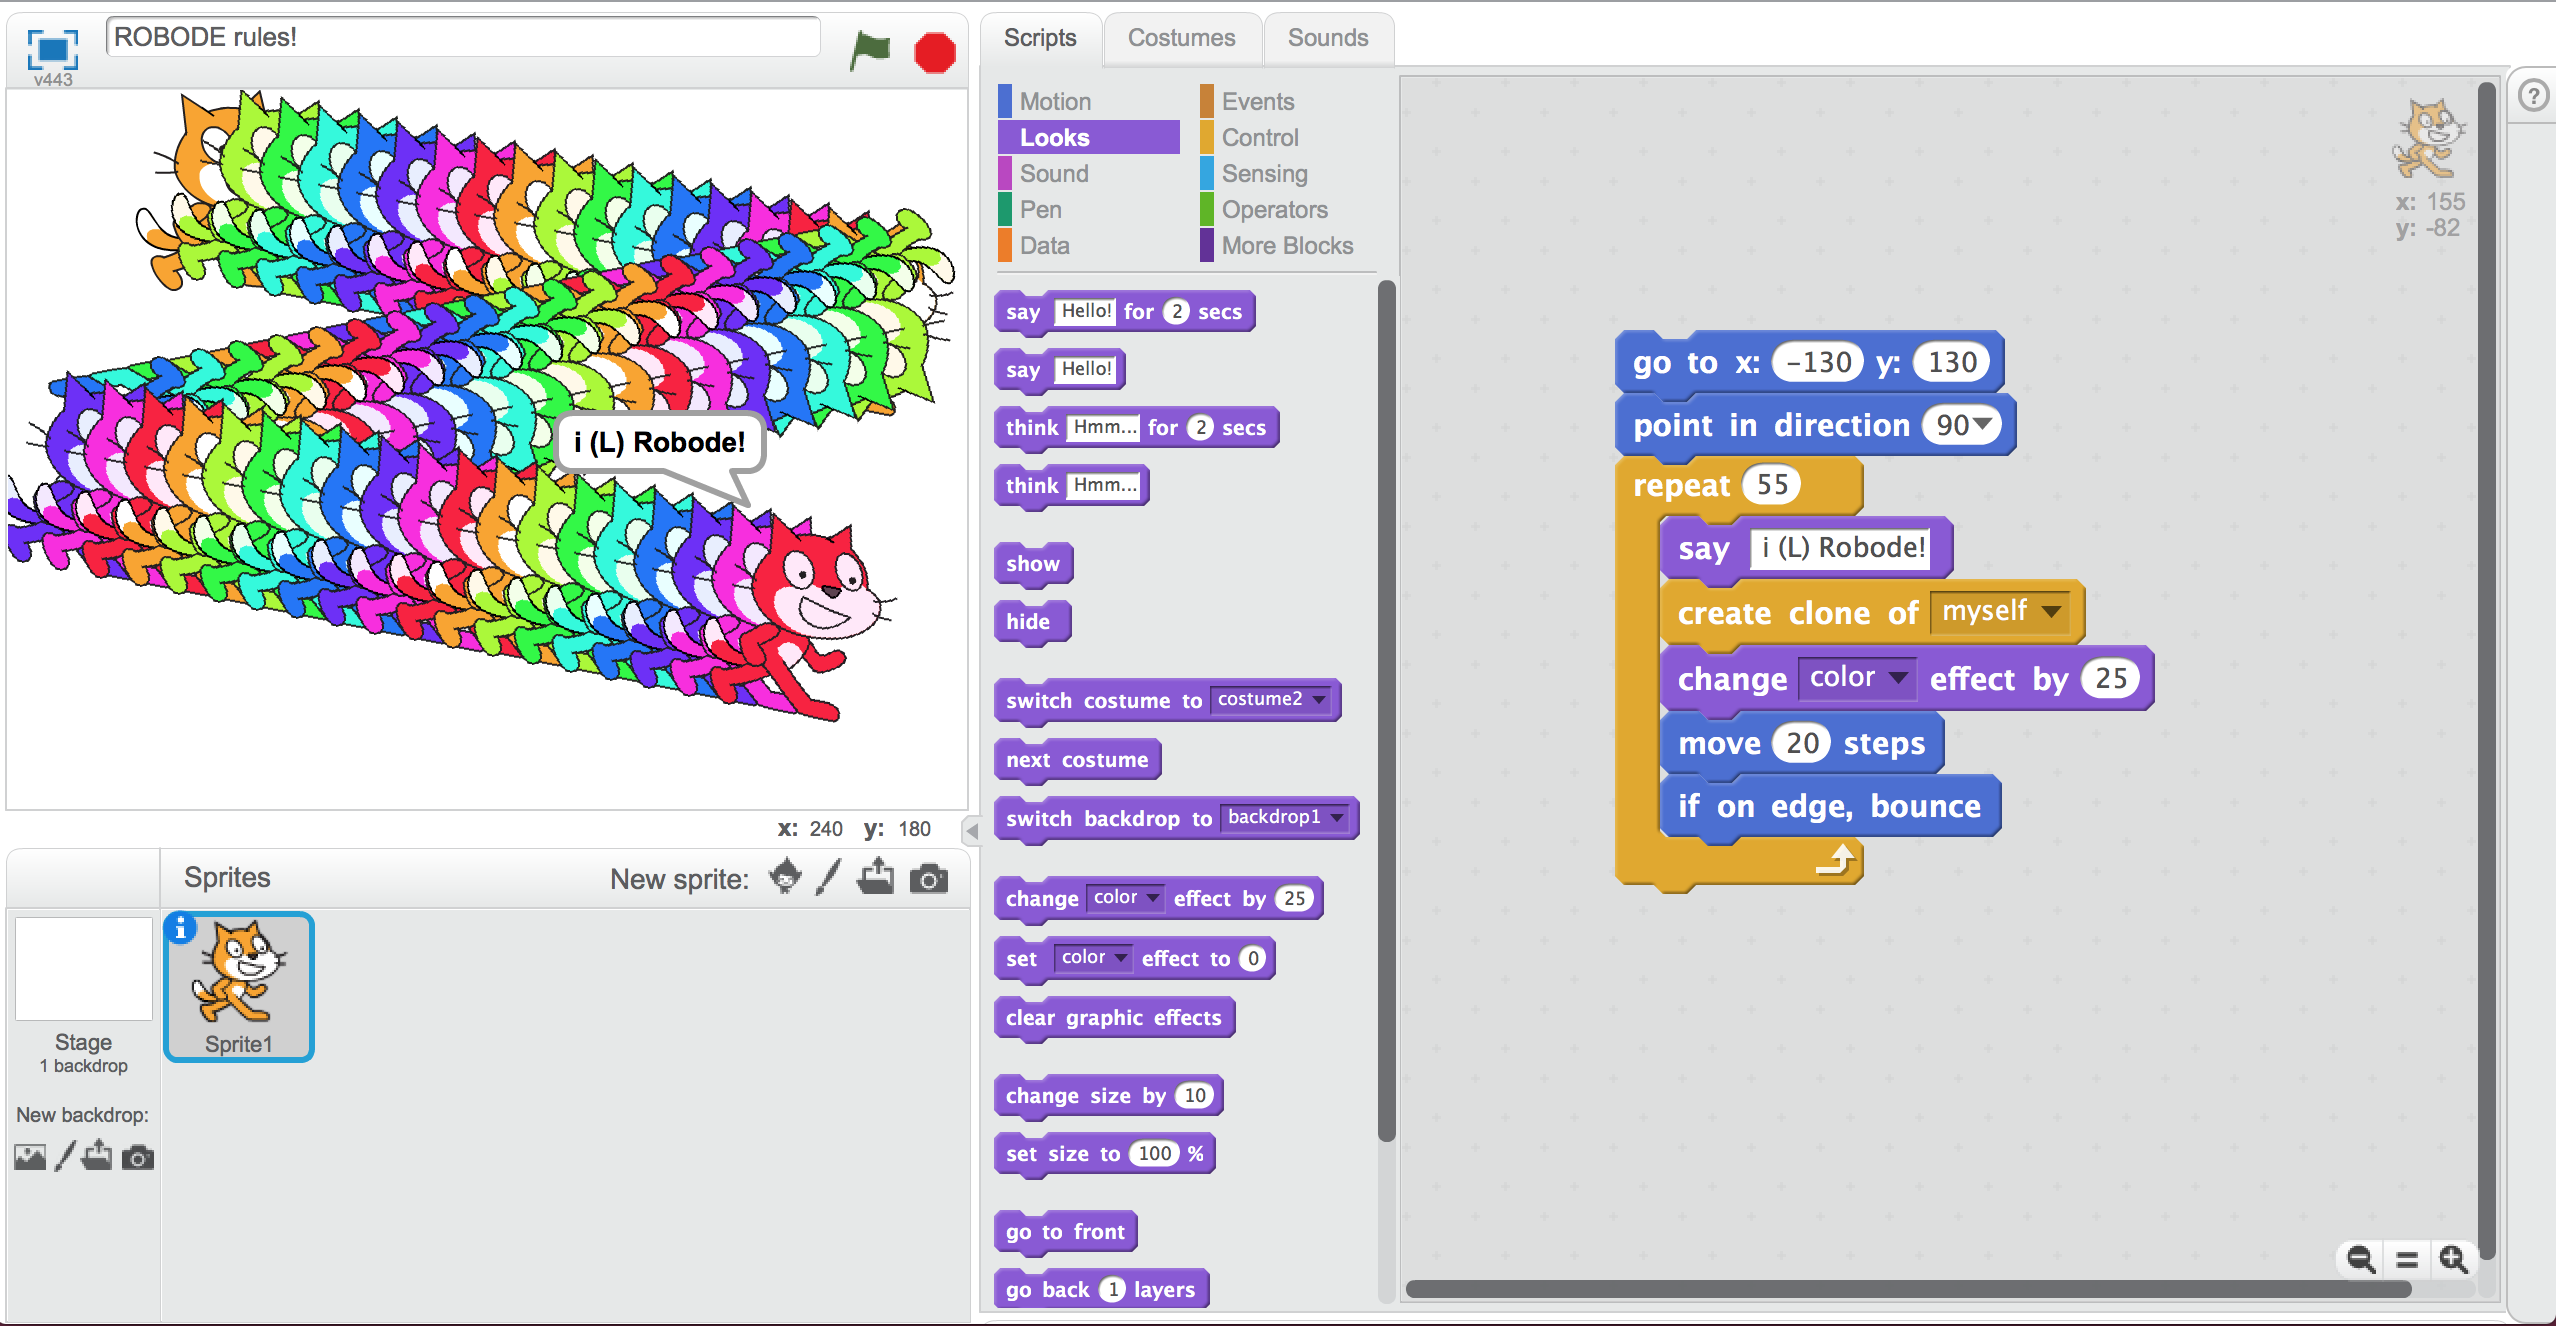
\includegraphics[width=1\textwidth]{images/scratch-example.png}
			\caption{Ejemplo de la interfaz de usuario y el editor de código que ofrece Scratch.}
				\label{fig:scratch-example}
	\end{centering}
\end{figure}

Cuando se programa con Scratch, la meta final es la de animar uno o más elementos por la pantalla. Estos elementos son los \emph{sprites} (imágenes), los cuales vienen predefinidos en una galería o pueden ser proporcionados por el propio usuario. Por tanto, los bloques irán enfocados a otorgar movimiento al \emph{sprite} en cuestión.

En cuanto a los tipos de bloques, actualmente están divididos en 11 categorías distintas:
\begin{itemize}
	\item \textbf{Movimiento:} Incluye funciones para mover, girar o establecer la posición y ángulo de giro del \emph{sprite}.
	\item \textbf{Apariencia:} Esta sección contiene funciones tanto para modificar la apariencia del \emph{sprite} como para mostrar mensajes en la pantalla a modo de diálogos de los \emph{sprites}.
	\item \textbf{Sonido:} Funciones para controlar el sonido de la aplicación que se está creando con Scratch. Permite reproducir sonidos precargados en la plataforma o subidos por el programador, diferentes instrumentos o establecer el volumen de la aplicación.
	\item \textbf{Pincel:} Permite pintar el escenario de forma similar a Turlte, dejando un rastro por donde se va desplazando (para más información sobre Turtle, consultar sección \ref{sec:turtle}).
	\item \textbf{Datos:} Creación de variables y listas y modificación de los valores de las mismas.
	\item \textbf{Eventos:} Bloques para detectar y reaccionar a ciertos eventos como el click de un ratón sobre un \emph{sprite} o el teclado.
	\item \textbf{Control:} Incluye bloques con las condiciones y bucles clásicos.
	\item \textbf{Percepción:} Esta sección contiene funciones para detectar eventos de teclado y ratón. También provee funciones para establecer lapsos de tiempo. 
	\item \textbf{Operadores:} Bloques para utilizar operadores matemáticos.
	\item \textbf{Bloques propios} y \textbf{Extensiones}: Scratch permite crear tus propios bloques y usar extensiones integradas con la aplicación como \emph{Lego WeDo} y \emph{PicoBoard}. 
\end{itemize}



%%%%%%%%%%%%%%%%%%%%%%%%%%%%%%%%%%%%%%%%%%%%%%%%
% Apendice F
%%%%%%%%%%%%%%%%%%%%%%%%%%%%%%%%%%%%%%%%%%%%%%%%
\chapter{Modificación de iJava para el simulador}
\label{anexo:ampliacion-ijava-API}

\section*{Cambio en el analizador semántico}

Estos cambios se han realizado en la clase \texttt{iJavaSemantic}, función \texttt{checkDeclaredFunctions()}. 

\begin{lstlisting}[language={Javascript},label={code:cambios-ijava-semantico}, caption={Código que muestra los cambios que se han realizado en la clase \texttt{iJavaSemantic} para cambiar la función principal \texttt{main} por \texttt{setup}.}]
function checkDeclaredFunctions() {
	var mainFound = false;
	for (var i = 0; i < declaredFunctions.length; i++) {
		//cambio la palabra clave "main" por "setup"
		if (declaredFunctions[i].id === "setup") {
			mainFound = true;
		}
		// (...)
	}
}
\end{lstlisting}

En el código \ref{code:ejemplo-eval-javascript} se muestra el código Javascript que se genera de la ejecución del código Javascript \ref{code:nuevo-modelo}


\begin{lstlisting}[language={Java},label={code:ejemplo-eval-javascript}, caption={Ejemplo de código Javascript que se genera cuando se ejecuta el código iJava \ref{code:nuevo-modelo}.}]
running = true;
var __setup = null;
var __loop = null;
var __delay = 0;
var __potenciaDer = 0;
var __potenciaIzq = 0;
var __setup = function() {
    __delay = 1000;
    __potenciaDer = 10;
    __potenciaIzq = 10;
    initRobot();
}
var __loop = function() {
    power(__potenciaIzq, __potenciaDer);
    wait(__delay);
    power(0, 0);
    wait(__delay * 2);
}

try {
    if (__setup) {
        __setup();
        if (__loop)
            animate(__loop);
    } else stop();
} catch (e) {
    error(e);
}
\end{lstlisting}

\section*{Cambios en el analizador sintáctico}

Los cambios en el analizador sintáctico corresponden a la clase \texttt{iJavaParser}. Es necesario añadir la definición de nuevas variables, funciones o símbolos del sistema en la función \texttt{init()}, que será la que los añada como parte del lenguaje. Se muestran el el siguiente código.


\begin{lstlisting}[language={Javascript},label={code:cambios-ijava-sintactico}, caption={Definición de las funciones y variables de la  API del simulador.}]
// Sensores de colisiones indivuduales
system_variable("sensorNW", BooleanDatatype, false);
system_variable("sensorNE", BooleanDatatype, false);
system_variable("sensorSW", BooleanDatatype, false);
system_variable("sensorSE", BooleanDatatype, false);

//sensores de lineas individuales
system_variable("sensorLR", BooleanDatatype, false);
system_variable("sensorLL", BooleanDatatype, false);

//sensores de colisión y lineas grupales
system_variable("collisioning", BooleanDatatype, false);

// wait (n_millisec)
library_function("wait", new FunctionDatatype(VoidDatatype, [{
	datatype: IntegerDatatype
}]));
//initRobot ()
library_function("initRobot", new FunctionDatatype(VoidDatatype, []));
//stopRobot()
library_function("stop", new FunctionDatatype(VoidDatatype, []));
//motors(vel_motor_izq, vel_motor_der)
library_function("power", new FunctionDatatype(VoidDatatype, [{
	datatype: IntegerDatatype
}, {
	datatype: IntegerDatatype
}]));
// left()
library_function("left", new FunctionDatatype(VoidDatatype, []));
\end{lstlisting}



\section*{Cambios en el Sandbox}


La implementación de las funciones y variables de la API se realizan en la clase \texttt{iJavaSandbox} y se pueden ver en el código siguiente:

\begin{lstlisting}[language={Javascript},label={code:cambios-ijava-sandbox}, caption={Implementación de las funciones y variables de la API en el Sandbox de iJava.}]
var roboderunning = false;

// sensors
var sensorNE = false,
    sensorNW = false,
    sensorSE = false,
    sensorSW = false;
var sensorLR = false,
    sensorLL = false;
var collisioning = false;


function wait(millis) {
    //Add delay time to runtime.timeLimit
    if (runtime) {
        if (runtime.deep > -1) {
            runtime.timeLimit[runtime.deep] += millis;
        }
    }

    var timestamp = (new Date()).getTime() + millis;
    while ((new Date()).getTime() < timestamp) {
        //do nothing
    }
}

function power(lspeed, rspeed) {

    if (!roboderunning) {
        var msg = {
            message: "Error: Primero es necesario iniciar el robot con la función: 'iniciarRobot()'."
        };
        error(msg);
        return;
    }

    var message = {
        fn: "move",
        params: [lspeed, rspeed]
    };
    sendMessage("robode", message);
}

function stop() {
    if (!roboderunning) {
        var msg = {
            message: "Error: Primero es necesario iniciar el robot con la función: 'iniciarRobot()'."
        };
        error(msg);
        return;
    }

    var message = {
        fn: "stop",
        params: []
    };
    sendMessage("robode", message);
}

function manageSensors(message) {
    switch (message.id) {
        case "sensorNW":
            sensorNW = (message.state === "begin");
            break;
        case "sensorNE":
            sensorNE = (message.state === "begin");
            break;
        case "sensorSW":
            sensorSW = (message.state === "begin");
            break;
        case "sensorSE":
            sensorSE = (message.state === "begin");
            break;
        case "sensorLR":
            sensorLR = (message.state === "begin");
            break;
        case "sensorLL":
            sensorLL = (message.state === "begin");
            break;
    }
    collisioning = sensorNW || sensorNE ||  sensorSW || sensorSE;
}
\end{lstlisting}






%%%%%%%%%%%%%%%%%%%%%%%%%%%%%%%%%%%%%%%%%%%%%%%%
% Apendice G
%%%%%%%%%%%%%%%%%%%%%%%%%%%%%%%%%%%%%%%%%%%%%%%%
\chapter{Creación de elementos en Box2D}
\label{anexo:creacion-elementos-box2d}


La creación de elementos (\emph{bodies}, \emph{fixtures}, \emph{joints}, etc) en Box2D utiliza un \emph{patrón factoría}, teniendo que definir primero en un objeto plantilla (definición) las características que tendrá el elemento a crear y luego diciéndole a \texttt{World} que cree dicho elemento a partir de la plantilla.

A continuación se explicarán las características principales de los elementos de Box2D y sus propiedades mas importantes.

\section*{Objeto \texttt{Body}}

Los cuerpos en Box2D pueden ser dinámicos (tipo \texttt{b2\_dynamicBody}) o estáticos (tipo \texttt{b2\_staticBody }). Un cuerpo dinámico podrá moverse y se verá afectado por el entorno y otros cuerpos. Un cuerpo estático será inmune a fuerzas como la gravedad y su posición no cambiará. Robode y todos sus componentes serán cuerpos dinámicos mientras que las fronteras del mundo, serán cuerpos estáticos. También, un cuerpo está activo si su propiedad \texttt{sleep} está activa. El efecto de un cuerpo inactivo ya se ha explicado en la sección \ref{sec:definicion-mundo}.

Un cuerpo conoce los \emph{fixtures} asociados a él (que puede ser más de uno) y los \emph{joints} a los que está atado.

Es el objeto \texttt{Body} el que contiene todas las propiedades físicas y que afectan al movimiento del mismo, como por ejemplo: la velocidad lineal y angular, el ángulo de rotación o la masa. Por supuesto, también la posición. Para obtener la posición de un cuerpo se utiliza el método \texttt{GetWorldCenter()} para obtener la posición en el mundo del centro de masas del cuerpo.


Las propiedades \texttt{linearDamping} y \texttt{angularDamping}\footnote{Aquí, con \emph{damping} se refiere al efecto de suelo mojado y el deslizamiento que un cuerpo tiene sobre una superficie, en especial cuando el cuerpo frena.} sirven para reducir la velocidad lineal y angular respectivamente cuando en el frenado.

%, y no con respecto al origen del mismo. Esto tiene que ver con las \emph{fixtures} que tenga asociadas dicho cuerpo. Por ejemplo, si un cuerpo tiene mas de una \emph{fixture}, la posición origen del cuerpo no representará la del 

 %ya que se puede definir la posición del cuerpo y la de la \emph{fixture} de manera que no coincidan. De esta manera, la función \texttt{GetWorldPosition()} obtendrá la posición correcta del cuerpo con respecto a la del \emph{fixture}.

Adicionalmente, se ha modificado el prototipo de las clases \texttt{b2Body} y \texttt{b2BodyDef} (clase plantilla para crear \emph{bodies}) para añadir una característica más al cuerpo, el nombre que se le asigna al cuerpo. Esto se usará principalmente para poder distinguir estos objetos fácilmente en una colisión.


\section*{Objeto \texttt{Fixture}}

Los objetos \texttt{b2Fixture} definen la apariencia del objeto al que están asociado y las características físicas que le harán interactuar con el mundo de una u otra manera.

Box2D proporciona dos clases principales para definir la forma de las \emph{fixtures}: \texttt{b2CircleShape()} y \texttt{b2PolygonShape()}. La primera representa a una forma circular y es necesario indicar el radio del circulo a crear. La segunda forma representa a un polígono. Los polígonos tienen dos formas principales de definirse:

\begin{itemize}
	\item Con forma de caja definiendo su ancho y largo (con el método \texttt{SetAsBox()}).
	\item Con una forma libre. Es necesario indicar los vértices del polígono y su cantidad (con el método \texttt{AsArray()}). Es así como se pueden crear triángulo o trapecios en Box2D, por ejemplo. En este caso es importante no crear formas cóncavas, pues provocarán errores en la simulación.
\end{itemize}


Además, un \emph{fixture} tiene propiedades de densidad, fricción y restitución que definirá la interacción de este con el mundo. La densidad es usada para calcular la masa del cuerpo al que está asociada la \emph{fixture}. La fricción se usa para hacer los cuerpos deslizarse de una manera realista. La restitución de un cuerpo es la elasticidad de este ante un impacto y según su valor, si rebota más o menos contra una superficie. 

Los valores de fricción y restitución oscilan entre 0 y 1. Siendo 0 la anulación de la propiedad y 1 el máximo valor que se le puede dar.


\section*{Objeto \texttt{Joint}}


Un \emph{Joint} es un elemento constrictor entre dos cuerpos, que controla el movimiento que hacen los cuerpos pegados por el joint. El punto por el que se une un cuerpo a un joint se denomina \emph{ancla}.

Hay distintos tipos de joints que limitan el movimiento de los cuerpos de diferentes maneras. A continuación se nombrarán los más importantes:

\begin{itemize}
	\item \texttt{Revolute} es un joint que fuerza a dos cuerpos a compartir el mismo \emph{ancla} con un cierto ángulo de libertad. También se puede configurar un \emph{motor} que hará girar el ancla y por tanto a los cuerpos.
	\item \texttt{Distance} es un joint que permite ata los cuerpos pero como si estuvieran sujetos a una cuerda. Los cuerpos tendrán una distancia máxima que se pueden separar (la longitud de la cuerda) pero no una mínima, pudiendo incluso chocar.
	\item \texttt{Prismatic} es un joint que simula el movimiento de un cuerpo unicamente sobre un eje de coordenadas, permitiendo movimientos como los de un ascensor.
\end{itemize}

En el simulador solo usaremos \emph{Joints} de tipo \emph{Revolute}, definidos por la clase \texttt{b2RevoluteJoint}.  En la inicialización del joint se deben indicar los dos cuerpos y el punto de ancla. También hay que establecer las propiedades relacionadas al motor (propiedad \texttt{enableMotor}), si se quiere que exista un límite de movimiento o no (propiedad \texttt{enableLimit}) y el valor máximo de torsión que se permite (propiedad \texttt{maxMotorTorque}).






%%%%%%%%%%%%%%%%%%%%%%%%%%%%%%%%%%%%%%%%%%%%%%%%
% Apendice H
%%%%%%%%%%%%%%%%%%%%%%%%%%%%%%%%%%%%%%%%%%%%%%%%
\chapter{Construcción de circuitos}
\label{sec:construccion-circuitos}

El circuito estará limitado por fronteras para prevenir que el robot se salga del mismo. La creación de las fronteras se puede ver en el código \ref{code:creacion-fronteras}.

\begin{lstlisting}[language={Javascript},label={code:creacion-fronteras}, caption={Función que crea las fronteras del mundo.}]
var scale = Simulator.config.scaleWorldIni;

var bodyDef = new Simulator.Env.b2BodyDef();
bodyDef.type = Simulator.Env.b2Body.b2_staticBody;
bodyDef.setName("border");

var fixDef = new Simulator.Env.b2FixtureDef();
fixDef.shape = new Simulator.Env.b2PolygonShape();

// lower border
fixDef.shape.SetAsBox(this.width / scale, 0.01);
bodyDef.position.Set((this.width / scale) / 2, this.height / scale);
Simulator.World.CreateBody(bodyDef).CreateFixture(fixDef);

// top border
bodyDef.position.Set((this.width / scale) / 2, 0);
Simulator.World.CreateBody(bodyDef).CreateFixture(fixDef);

// right border
fixDef.shape.SetAsBox(0.01, this.height / scale);
bodyDef.position.Set(this.width / scale, (this.height / scale) / 2);
Simulator.World.CreateBody(bodyDef).CreateFixture(fixDef);

// left border
bodyDef.position.Set(0, (this.height / scale) / 2);
Simulator.World.CreateBody(bodyDef).CreateFixture(fixDef);
\end{lstlisting}

La posición y tamaño de las fronteras se crearán en función de la escala inicial del mundo. Por otra parte, las fronteras se definirán como objetos \texttt{b2\_staticBody} para que permanezcan inmutables en nuestro mundo.

Un obstáculo se crearía de manera similar a como se han creado los ruedas o el cuerpo principal.

%\color{green} ===CREAR UN CIRCUITO===}.
